% \documentclass[linenumbers,floatfix,ApJL,twocolumn]{aastex631}
\documentclass[floatfix,ApJL,twocolumn]{aastex631}

\usepackage{amssymb}
\usepackage{amsmath}
\usepackage{microtype}
\usepackage{url}
\usepackage{xspace}
\usepackage{xcolor}
\usepackage{ifxetex}
\ifxetex
\usepackage{fontspec}
\defaultfontfeatures{Extension = .otf}
\fi
\usepackage{fontawesome}



\setlength{\parindent}{3.0ex}


% Projects:
\newcommand{\project}[1]{\textsf{#1}}

\newcommand{\python}{\project{Python}}
\newcommand{\cython}{\project{Cython}}
\newcommand{\cpp}{\project{C++}}
\newcommand{\jupyter}{\project{Jupyter}}

\newcommand{\exoplanet}{\project{exoplanet}}
\newcommand{\lightkurve}{\project{lightkurve}}
\newcommand{\starry}{\project{starry}}
\newcommand{\theano}{\project{Theano}}
\newcommand{\pymc}{\project{PyMC3}}
\newcommand{\celerite}{\project{celerite}}
\newcommand{\dynesty}{\project{dynesty}}
\newcommand{\astroquery}{\project{astroquery}}
\newcommand{\scipy}{\project{scipy}}
\newcommand{\jupytext}{\project{jupytext}}
\newcommand{\sphinx}{\project{sphinx}}
\newcommand{\jupyterbook}{\project{Jupyter-book}}
\newcommand{\arviz}{\project{ArviZ}}
\newcommand{\nbconvert}{\project{nbconvert}}


\newcommand{\tess}{\project{TESS}}
\newcommand{\kepler}{\project{Kepler}}
\newcommand{\gaia}{\project{Gaia}}

\newcommand{\mast}{\project{MAST}}
\newcommand{\exofop}{\project{ExoFOP}}

\newcommand{\tessAtlas}{\project{TESS Atlas}}

% math
\newcommand{\T}{\ensuremath{\mathrm{T}}}
\newcommand{\dd}{\ensuremath{ \mathrm{d}}}
\newcommand{\unit}[1]{{\ensuremath{ \mathrm{#1}}}}
\newcommand{\bvec}[1]{{\ensuremath{\boldsymbol{#1}}}}


\DeclareMathOperator{\invG}{Inv-\mathnormal{\Gamma}}
\DeclareMathOperator{\N}{\mathcal{N}}
\DeclareMathOperator{\U}{\mathcal{U}}
\DeclareMathOperator{\Un}{\mathcal{U}}
\DeclareMathOperator{\Par}{\mathcal{P}ar}
\DeclareMathOperator{\tmin}{\mathnormal{t_{\rm min}}}
\DeclareMathOperator{\tmax}{\mathnormal{t_{\rm max}}}





%% affiliation shortcuts
\newcommand{\SPA}{School of Physics and Astronomy, Monash University, Clayton VIC 3800, Australia}
\newcommand{\OzGravMonash}{OzGrav: The ARC Centre of Excellence for Gravitational Wave Discovery, Clayton VIC 3800, Australia}
\newcommand{\AMNH}{Department of Astrophysics, American Museum of Natural History, New York, NY 10024, USA}
\newcommand{\CCA}{Center for Computational Astrophysics, Flatiron Institute, New York, NY 10010, USA}
\newcommand{\CUNY}{Graduate Center, City University of New York, 365 5th Avenue, New York, NY 10016, USA}
\newcommand{\BMCC}{Department of Science, BMCC, City University of New York, New York, NY 10007, USA}





\newif\ifdraft
\drafttrue % switch to false in non-draft version (thereby hiding the todos)
\newcommand{\inDraftVersion}[1]{\ifdraft #1\fi} 


% TODOs
\newcommand{\todo}[3]{\inDraftVersion{{\color{#2}\emph{#1}: #3}}}
\newcommand{\dfmtodo}[1]{\todo{DFM}{red}{#1}}
\newcommand{\avi}[1]{\todo{Avi}{red}{#1}}
\newcommand{\alltodo}[1]{\todo{TODO}{red}{#1}}
\newcommand{\citeme}{{\color{red}(citation needed)}}


\newcommand{\red}{\textcolor{red}}
\newcommand{\textuit}[1]{\textit{\underline{#1}}}



%% Numbers
% https://exoplanetarchive.ipac.caltech.edu/docs/counts_detail.html
% https://exoplanetarchive.ipac.caltech.edu/index.html

\newcommand{\numConfirmedPlanets}{5,090} % 
\newcommand{\numCandidatesRemaining}{6,959}

\newcommand{\numTessCandidates}{5,488} % 
\newcommand{\numTessPlanets}{227}
\newcommand{\numAnalysed}{2,833}
\newcommand{\numAnalysedMulti}{151}
\newcommand{\numAnalysedSingle}{68}
\newcommand{\cpuHrs}{$\sim80,000\ \rm{Hrs}$}

%% links

% % % from: https://github.com/rodluger/corTeX
% % % Add code, proof, and animation hyperlinks
% \definecolor{linkcolor}{rgb}{0.1216,0.4667,0.7059}
% \newcommand{\codeicon}{{\color{linkcolor}\faFileCodeO}}

% % % Define the `oscaption` command for open source figure captions
% \newcommand{\oscaption}[2]{\caption{#2 \codelink{#1}}}


% \makeatletter
\newcommand{\github}[1]{\href{#1}{\textcolor{gray}{\faGithubSquare}}}








\shorttitle{The \tess\ Atlas}


\begin{document}

\title{The \tess\ Atlas: an open source catalog of TESS transit fits}

\correspondingauthor{Daniel Foreman-Mackey}
\email{foreman.mackey@gmail.com}

\author[0000-0002-4146-1132{Avi Vajpeyi}
\affiliation{
    School of Physics and Astronomy,
    Monash University,
    Clayton VIC 3800,
    Australia
}
\affiliation{
OzGrav: The ARC Centre of Excellence for Gravitational Wave Discovery,
Clayton VIC 3800,
Australia
}

\author[0000-0002-9328-5652]{Daniel Foreman-Mackey}
\affiliation{
    Center for Computational Astrophysics,
    Flatiron Institute,
    162 5th Ave,
    New York, NY 10010
}







\begin{abstract}
% The Transiting Exoplanet Survey Satellite \tess\ has enabled the discovery of more than five-thousand exoplanet candidates, out of which only a few hundred have been confirmed.
% Exoplanet confirmation requires vetting of candidates by ruling out false positives and follow-up observations and analyses.
We present the \tess\ Atlas, a catalog of candidate exoplanet parameter estimates, from two-minute cadence \tess\  data, to assist the vetting process and follow-up analyses.
This catalog contains posterior estimates for \red{\numAnalysed} \tess\ Objects of Interest, including \red{\numAnalysedMulti} multi-planet candidate systems and \red{\numAnalysedSingle} candidates having data for a single transit.
Our analysis utilises the No-U-Turns Markov chain Monte Carlo algorithm to sample the parameter space with a circular transit model implemented in \exoplanet.
\avi{The \tess\ Atlas estimates are different from the ExoFop}.
We provide posterior samples from our analyses and \jupyter notebooks to reproduce the analyses for each exoplanet candidate.
\end{abstract}

% info on sectors: https://heasarc.gsfc.nasa.gov/docs/tess/sector.html

\keywords{%
  methods: data analysis ---
  methods: statistical ---
  miscellaneous --- catalogs --- surveys
}


\section{Introduction} \label{sec:intro}

In March 2022, NASA's exoplanet archive~\citep{Akeson:2013:PASP}\footnote{\href{https://exoplanetarchive.ipac.caltech.edu/}{https://exoplanetarchive.ipac.caltech.edu/}} surpassed five thousand confirmed exoplanets, a milestone made possible by data from several observatories, including the Transiting Exoplanet Survey Satellite TESS~\citep{Ricker:2015:JATIS}.
The confirmed exoplanets exhibit a wide range of masses, compositions, and radii.
Some of these planets are also located within their planetary systems' habitable zone.
Furthermore, the population of these exoplanets has fuelled research into planetary system architecture, planetary formation and evolution, and updated exoplanet occurrence rates.
These analyses will be more informative with a bigger sample of exoplanets and more precise estimates of the planet's characteristics.
This list of ~5000 exoplanets may be dramatically increased once the 6000 exoplanets awaiting validation are processed, more than half of which are candidates detected in TESS data.
The majority of TESS exoplanet candidates were discovered using the photometric transit method.
Unfortunately, systematic effects (e.g. ) and non-planetary astrophysical sources (e.g. stellar granulation and eclipsing binaries) can mimic exoplanet transits.
Hence, to validate these candidates, it is necessary to eliminate false positives and, if possible, conduct additional observations. 

Targets are assigned consecutive TOI IDs. Multi- planet systems are assigned suffixes (.01, .02, etc.) mir- roring the suffixes assigned for the TCE. TEV automat- ically generates a comma-separated values (CSV) file with all necessary parameters for each TOI from the vetted TOI list. Each TOI has a table of pa- rameters, a DV summary page, and a full DV report.


This motivates constructing a homogeneous method of \tess\ Atlas, a catalog of transiting exoplanet posterior estimates for the \red{\numAnalysed} \tess\ Objects of Interest (TOIs) with two-minute cadence observations from 2018 through 2022.
The catalog of posteriors, summary statistics, and software to reproduce the analyses are provided at \atlasUrl.
The website contains a \jupyter notebook for each TOI, documenting the end-to-end analysis of each TOI.
The notebooks contain software to download and clean light curve data, the transit model and priors for inference implementations, the \pymc sampling stage, and a posterior post-processing step.
The website also documents the method to download our Bayesian parameter inference posterior samples, load them and make various plots.


We provide software to reproduce the analyses and results at \atlasUrl.
The website contains one Jupyter notebook for each TOI, demonstrating the end-to-end analysis of a TOI.
The notebooks contain software to download and clean light curve data, implementations of the transit-model and priors for inference, the \pymc sampling stage, and a posterior post-processing step.
The website also documents the method to download our Bayesian parameter inference posterior samples, load them and make various plots.


The remainder of the paper is organised as follows: Section~\ref{sec:method} describes our transit light curve model and the Bayesian framework we use to estimate parameters of exoplanet systems from the observed data.
The analysis results are summarised in Section~\ref{sec:results}.
The catalog, released data, and software to reproduce the results are described in Section~\ref{sec:data} and are available online as supplementary materials (\atlasUrl).
Finally, we provide concluding remarks in Section~\ref{sec:conclusion}.

\section{Method} \label{sec:method}

In this section, we outline the procedures to analyse each TOI and generate the \tessAtlas. 


\subsection{Target selection and setup }

\begin{figure*}
    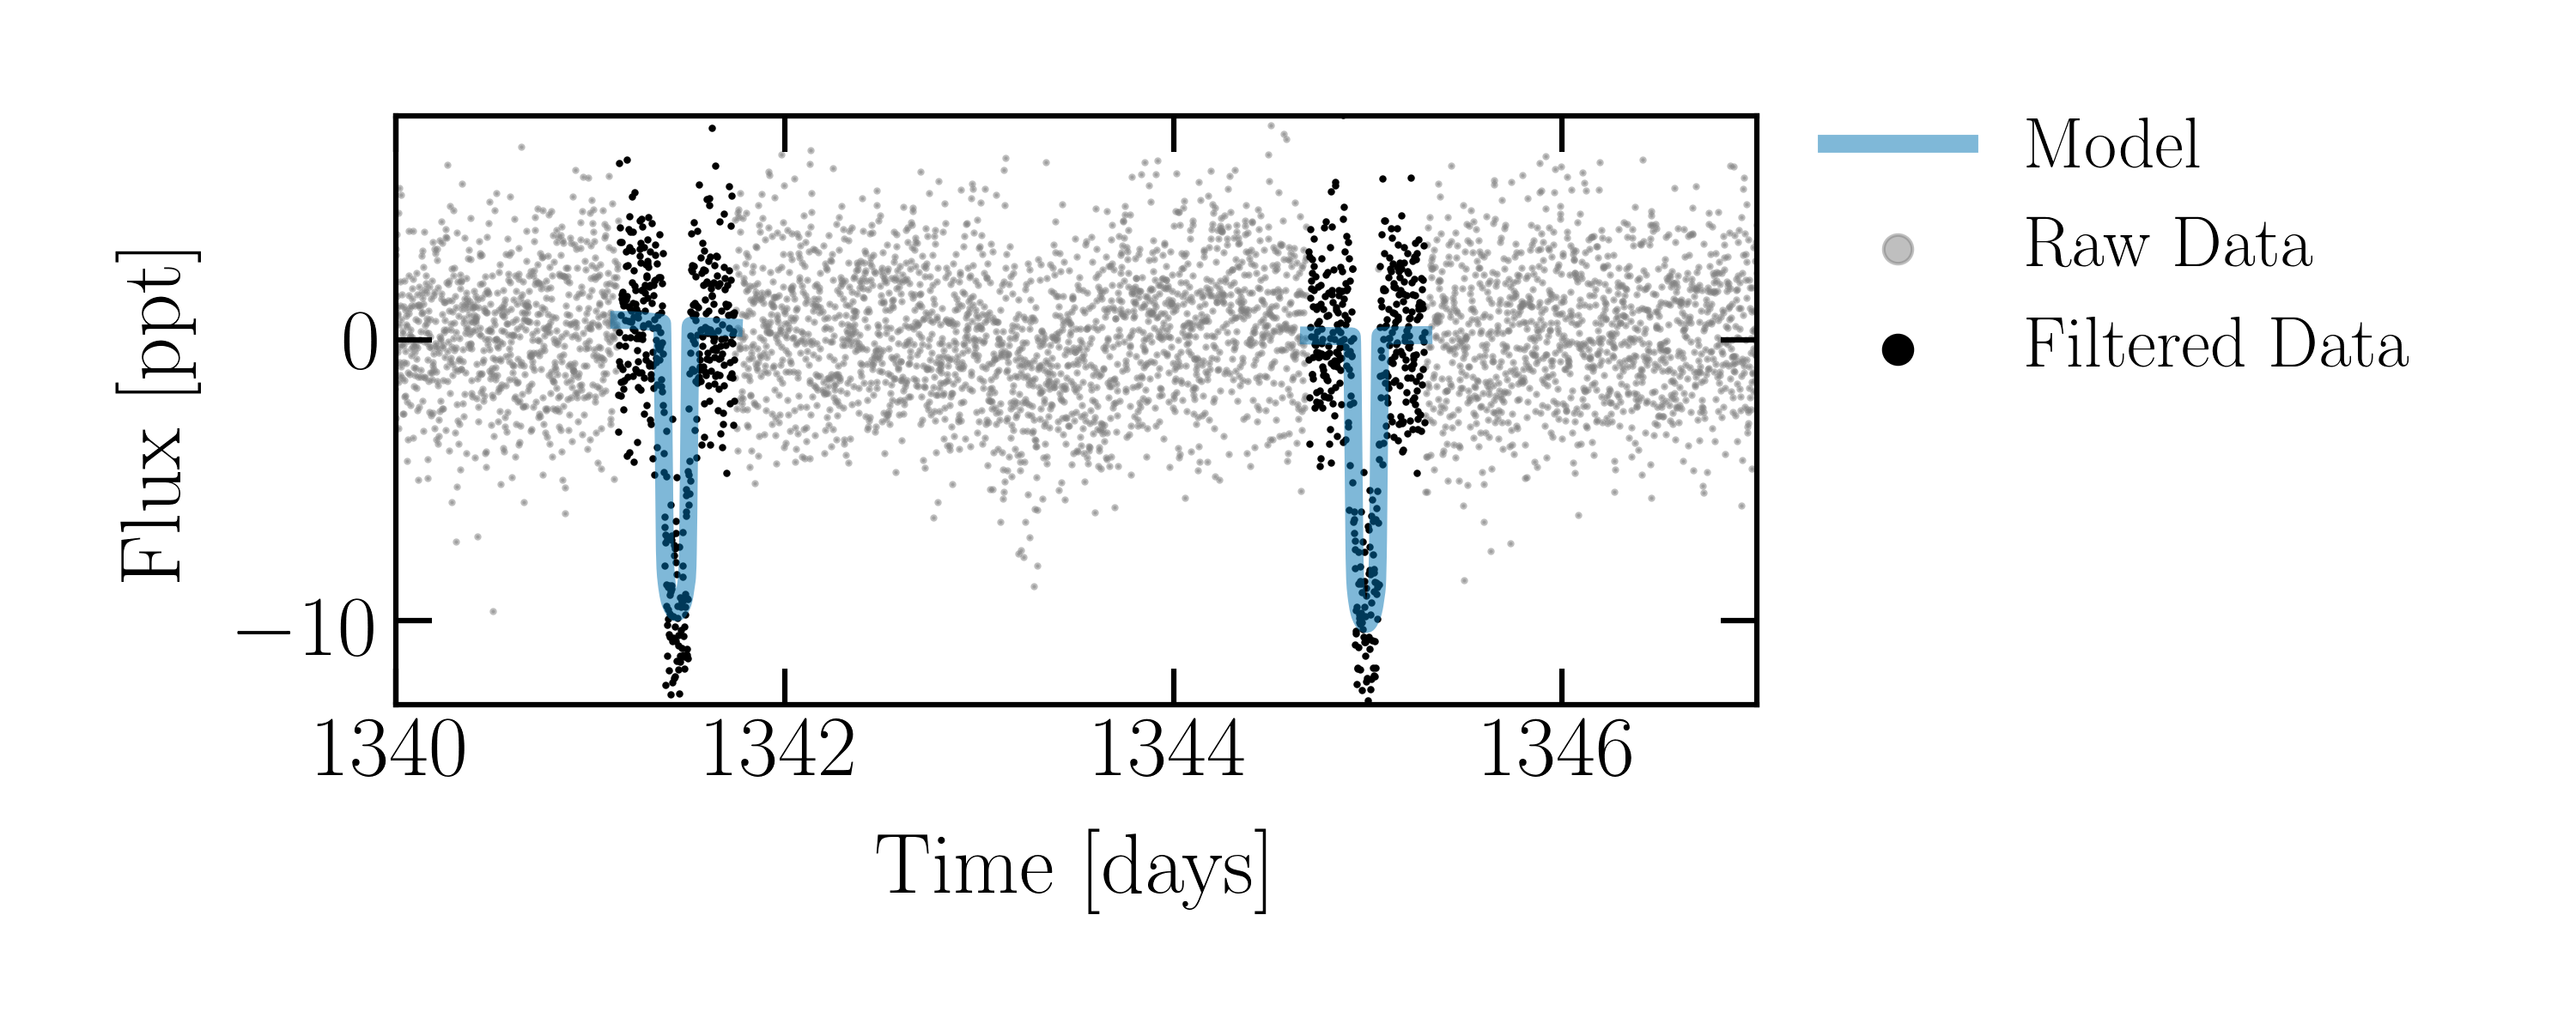
\includegraphics[width=\linewidth]{figures/raw_data_toi_103.png}
    \caption{\textbf{Light curve data for TOI-103 (from 1030-1450 BKJD):} The raw light curve data for TOI 103 is plotted in gray points, with \exofop\ best transit model parameter fit plotted on top in blue. The black points are obtained by filtering the raw data using the \exofop\ transit parameter estimates as described in the text. Code to reproduce this plot can be found on GitHub. \avi{TBH, maybe we should allow for more data?? What is the point of such wide priors if this is so tight. We should either base the cuts on the tmin and tmax priors, or make the tmin and tmax priors narrower.}}
    \label{fig:}
\end{figure*}


We obtain planetary parameters for \numTessCandidates TOIs with two-minute cadence data (as of Sept 2022) from the Exoplanet Follow-up Observing Program for TESS (ExoFOP-TESS) catalog.
This catalog reflects the best possible analysis available at the time of vetting.
Using \lightkurve\ we download the light curves for these TOIs generated by the TESS Science Processing Operations Center pipeline (Twicken et al. 2016; Jenkins 2020, SPOC), and stored ins the Mikulski Archive for Space Telescopes (\mast) at the Space Telescope Science Institute.

As a pre-processing step, low-frequency outliers are filtered from the light curve by removing data points with a root-mean-square (RMS) value above five when subtracted to a \scipy’s Savitzky-Golay filter (with a window length of 11 and sigma of 100) version of the light curve. 
Furthermore, we assume that the \exofop\ period and phase of the orbit are well measured and fit only the data nearby the anticipated transit times (with a buffer of buffer $\pm2\tau$ around the transit times) and disregard the remaining light curve data. 
A plot of the raw \mast light curve data obtained for {TOI 103}, along with the filtered data based on the transit time provided by \exofop\ is shown in Figure~\ref{fig:raw}.
Finally, if available, estimates for each TOIs host star's mass, radius and stellar density are downloaded from \mast. 



\subsection{Transit Model}

We model exoplanet transits as circular (non-interacting) Keplerian orbits around their host star, using \exoplanet~\citep{Foreman-Mackey:2021:JOSS}. 
Circular orbits permit the use of computationally efficient, analytical orbital dynamics calculations.
Additionally, circular orbits avoid degeneracies between eccentricity $e$, the argument of periastron $\omega$, impact parameter $b$, and planet radius $R_p$. 
Furthermore, the eccentricity can also be computed in post-processing, as described by \citet{Dawson:2012:ApJ}.
Each of the $n$ exoplanets in a system is parameterised by the planets'
\begin{enumerate}
  \item \emph{two reference transit times}, one near the beginning of the observations, $t_{\rm min}[n]$, and one near the end, $t_{\rm max}[n]$, both measured in \tess\ BJD,
  \item \emph{the transit duration} $\tau[n]$, measured in hours,
  \item \emph{the impact parameter} of the orbit, $b[n]$, constrained to be $|b| \le 1$,
  \item \emph{the radius ratio} $k[n]=R_{\rm p}[n] / R_\star$, of the planet radius $R_{\rm p}[n]$ divided by the stellar radius $R_\star$, and
  \item \emph{the approximate transit depth} $\delta[n]$, measured in parts-per-thousand.
\end{enumerate}
In the case that a planet has only a single transit in the data, the second reference time $t_{\rm max}[n]$ is substituted with the planet's orbital period $P[n]$
The host star's limb darkening profile is approximated using \citet{Kipping:2013:MNRAS}'s quadratic limb darkening law \citep{Claret:2000:A&A, Mandel:2002:ApJL}, parameterised in \starry~\citep{Luger:2019:AJ} by the baseline relative flux of the light curve $f_0$ and two quadratic limb-darkening parameters $u_1, u_2$.
Finally, stellar variability (from e.g. asteroseismic oscillation of the star)  is modelled with a \celerite~\citep{Foreman-Mackey:2017:ascl} Gaussian Process (GP), with a stochastically driven damped harmonic oscillator kernel in linear combination with a jitter term, to capture misspecified error bars and model misspecification.
The GP requires three parameters: the quality factor $Q_{\rm GP}$, the undamped period of the oscillator $\rho_{\rm GP}$, and the standard deviation of the process $\sigma_{\rm GP}$. 
More details of this transit parameterisation are presented in Appendix~\ref{apdx:model_details}. 
Implementation details for the various model components are available on the \exoplanet\ documentation website. 

\subsection{Inference Framework}

Uninformative priors are set for the stellar limb darkening, mean flux, and noise parameters. 
While the transiting exoplanet parameter priors are centred around the \exofop\ estimates, the priors are given wide ranges to allow adequate parameter space exploration.
A full list of the priors used is presented in Table~\ref{}. 
Note that we use a joint prior on radius ratio and impact parameter, implemented in \exoplanet's \textsc{ImpactParameter}, that produces flat marginal priors for both parameters. 

The posterior sampler's starting point is initialised at a high likelihood point by utilising \exoplanet's non-linear optimisation framework provided.
After initial optimisation, the posterior distribution is sampled using a Hamiltonian Monte Carlo (HMC) No U-Turn Sampler with \pymc~\citep{}.
The sampler is run on two chains for 4,000 steps with a burn-in of 2,000 steps.
We pass the two chains to \arviz\ to compute rank normalised $\hat{R}$ diagnostic statistic~\cite{Vehtari:2019:arXiv} and flag analyses with $\hat{R}>1.01$ to have convergence issues. 

For successful analyses, we conduct a post-processing step to compute the orbital eccentricity and argument of periapsis for each transiting planet. 
The transit light curve observables such as the transit duration depend degenerately on the eccentricity and hosts star's density~\citep{Dawson:2012:ApJ}. 
So, using our measurements of transit observables, we can approximate the stellar density and an independent measurement of stellar density to reweight posterior samples 
 Therefore, if the transit is fit using stellar density (or duration, in this case) as one of the parameters, it is possible to make an independent measurement of the stellar density, and in turn, infer the eccentricity of the orbit as a post-processing step. The details of this eccentricity calculation method are described in Dawson n Johnson (2012).

\subsection{Analysis execution and website generation}

All the analysis steps for a TOI, from data retrieval to post-processing, are implemented in a `template' python script that can be converted into a \jupyter notebook with \jupytext~toiTemplateLink~\cite{}.
After duplicating the template for each TOI, we insert the TOI number in the notebooks and execute them in parallel with `nbconvert'. 
Once analysis is complete, we use \jupyterbook, a package built upon \sphinx\ and \nbconvert\   to convert the pre-processed notebooks with the various plots, into `html' webpages, which are then deployed online on the \tessAtlas\ website. 
Additionally, the raw data used for analysis (the light curve data and \exofop\ estimates) and the analysis data products (the HMC chains and reweighted posteriors) are uploaded and made publicly accessible. 


\section{Results}\label{sec:results}



\begin{figure*}
    \gridline{
        \fig{figures/planet_3_posterior.png}{0.5\linewidth}{}
        \fig{figures/ecc_3_posterior.png}{0.3\linewidth}{}
    }
    \caption{\textbf{Main caption:} stuff }
    \label{fig:}
\end{figure*}


\begin{figure}
    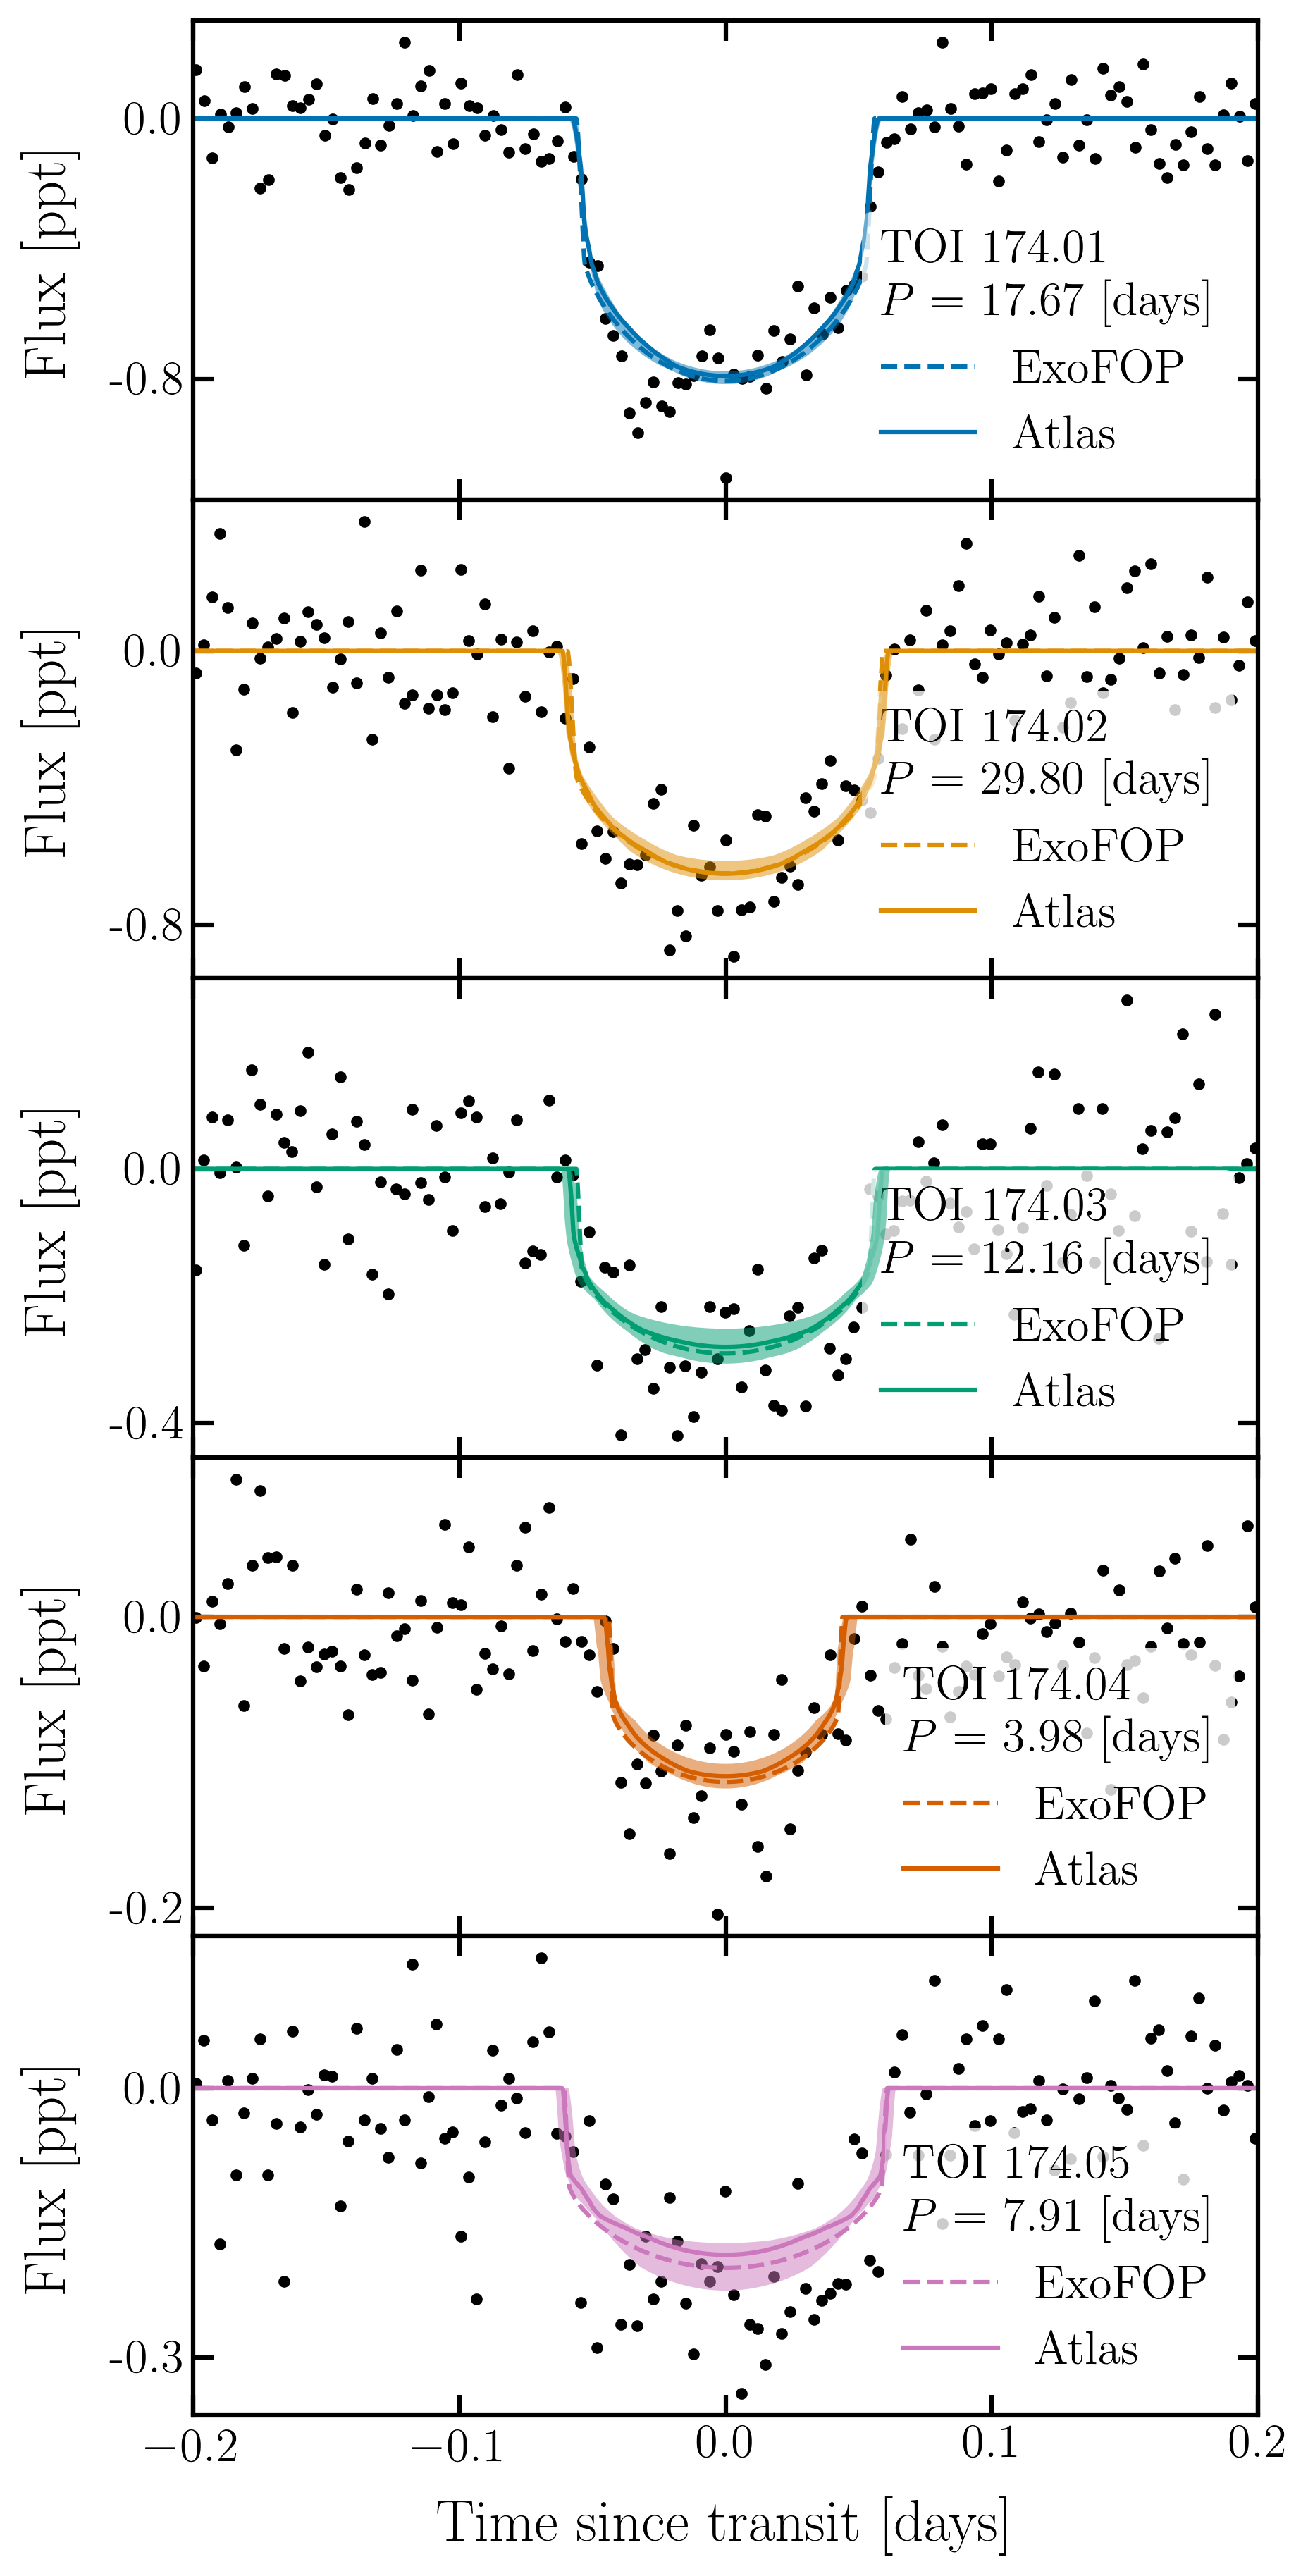
\includegraphics[width=0.9\linewidth]{paper/figures/toi_174_phase.png}
    \caption{\textbf{Main caption:} stuff }
    \label{fig:}
\end{figure}


Our analysis of individual planets show posterior and phase plots


Our bulk table of parameter estimates.







To provide context for our planet candidates in regard to
planet demographics and the radius valley, we display our
planet candidates in the planet radius–period space, and compare them with nearby candidates from the TOI and DIAmante catalogs, together with additional confirmed transiting planets observed in



\begin{figure}
  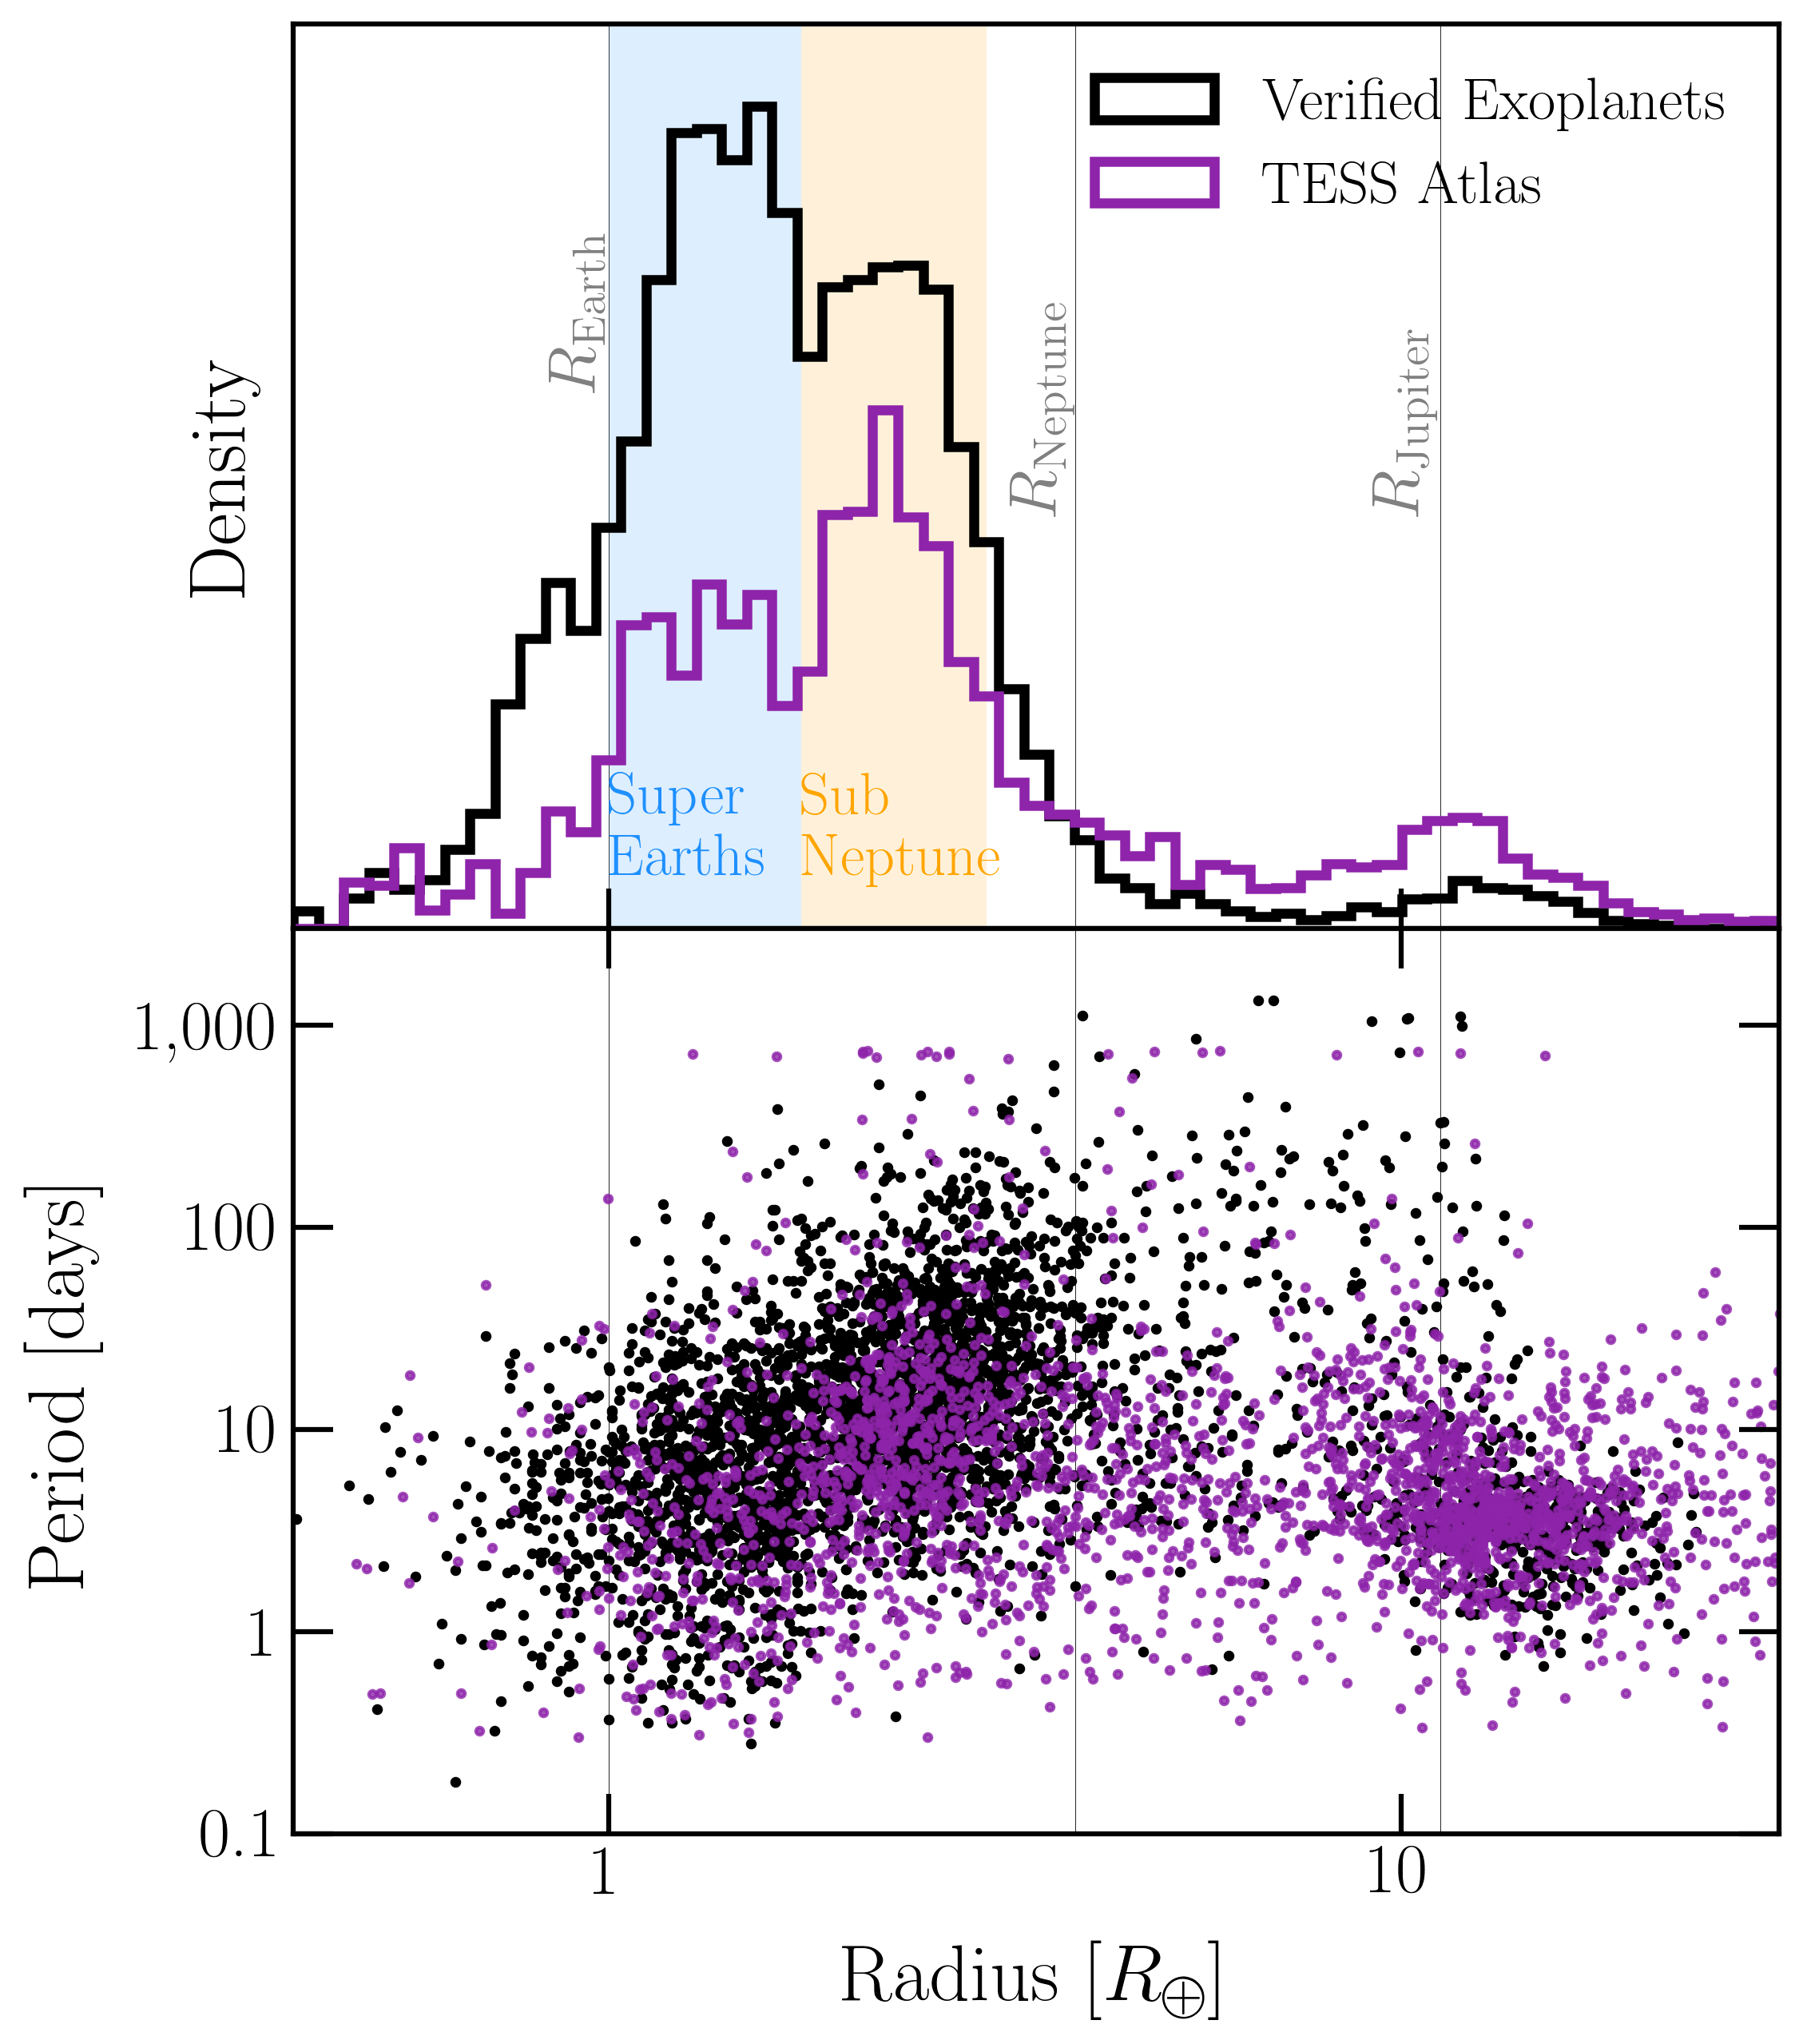
\includegraphics[width=\linewidth]{figures/radius_period_plot.png}
  \caption{\textbf{Main caption:} stuff }
  \label{fig:}
\end{figure}


\begin{figure}
  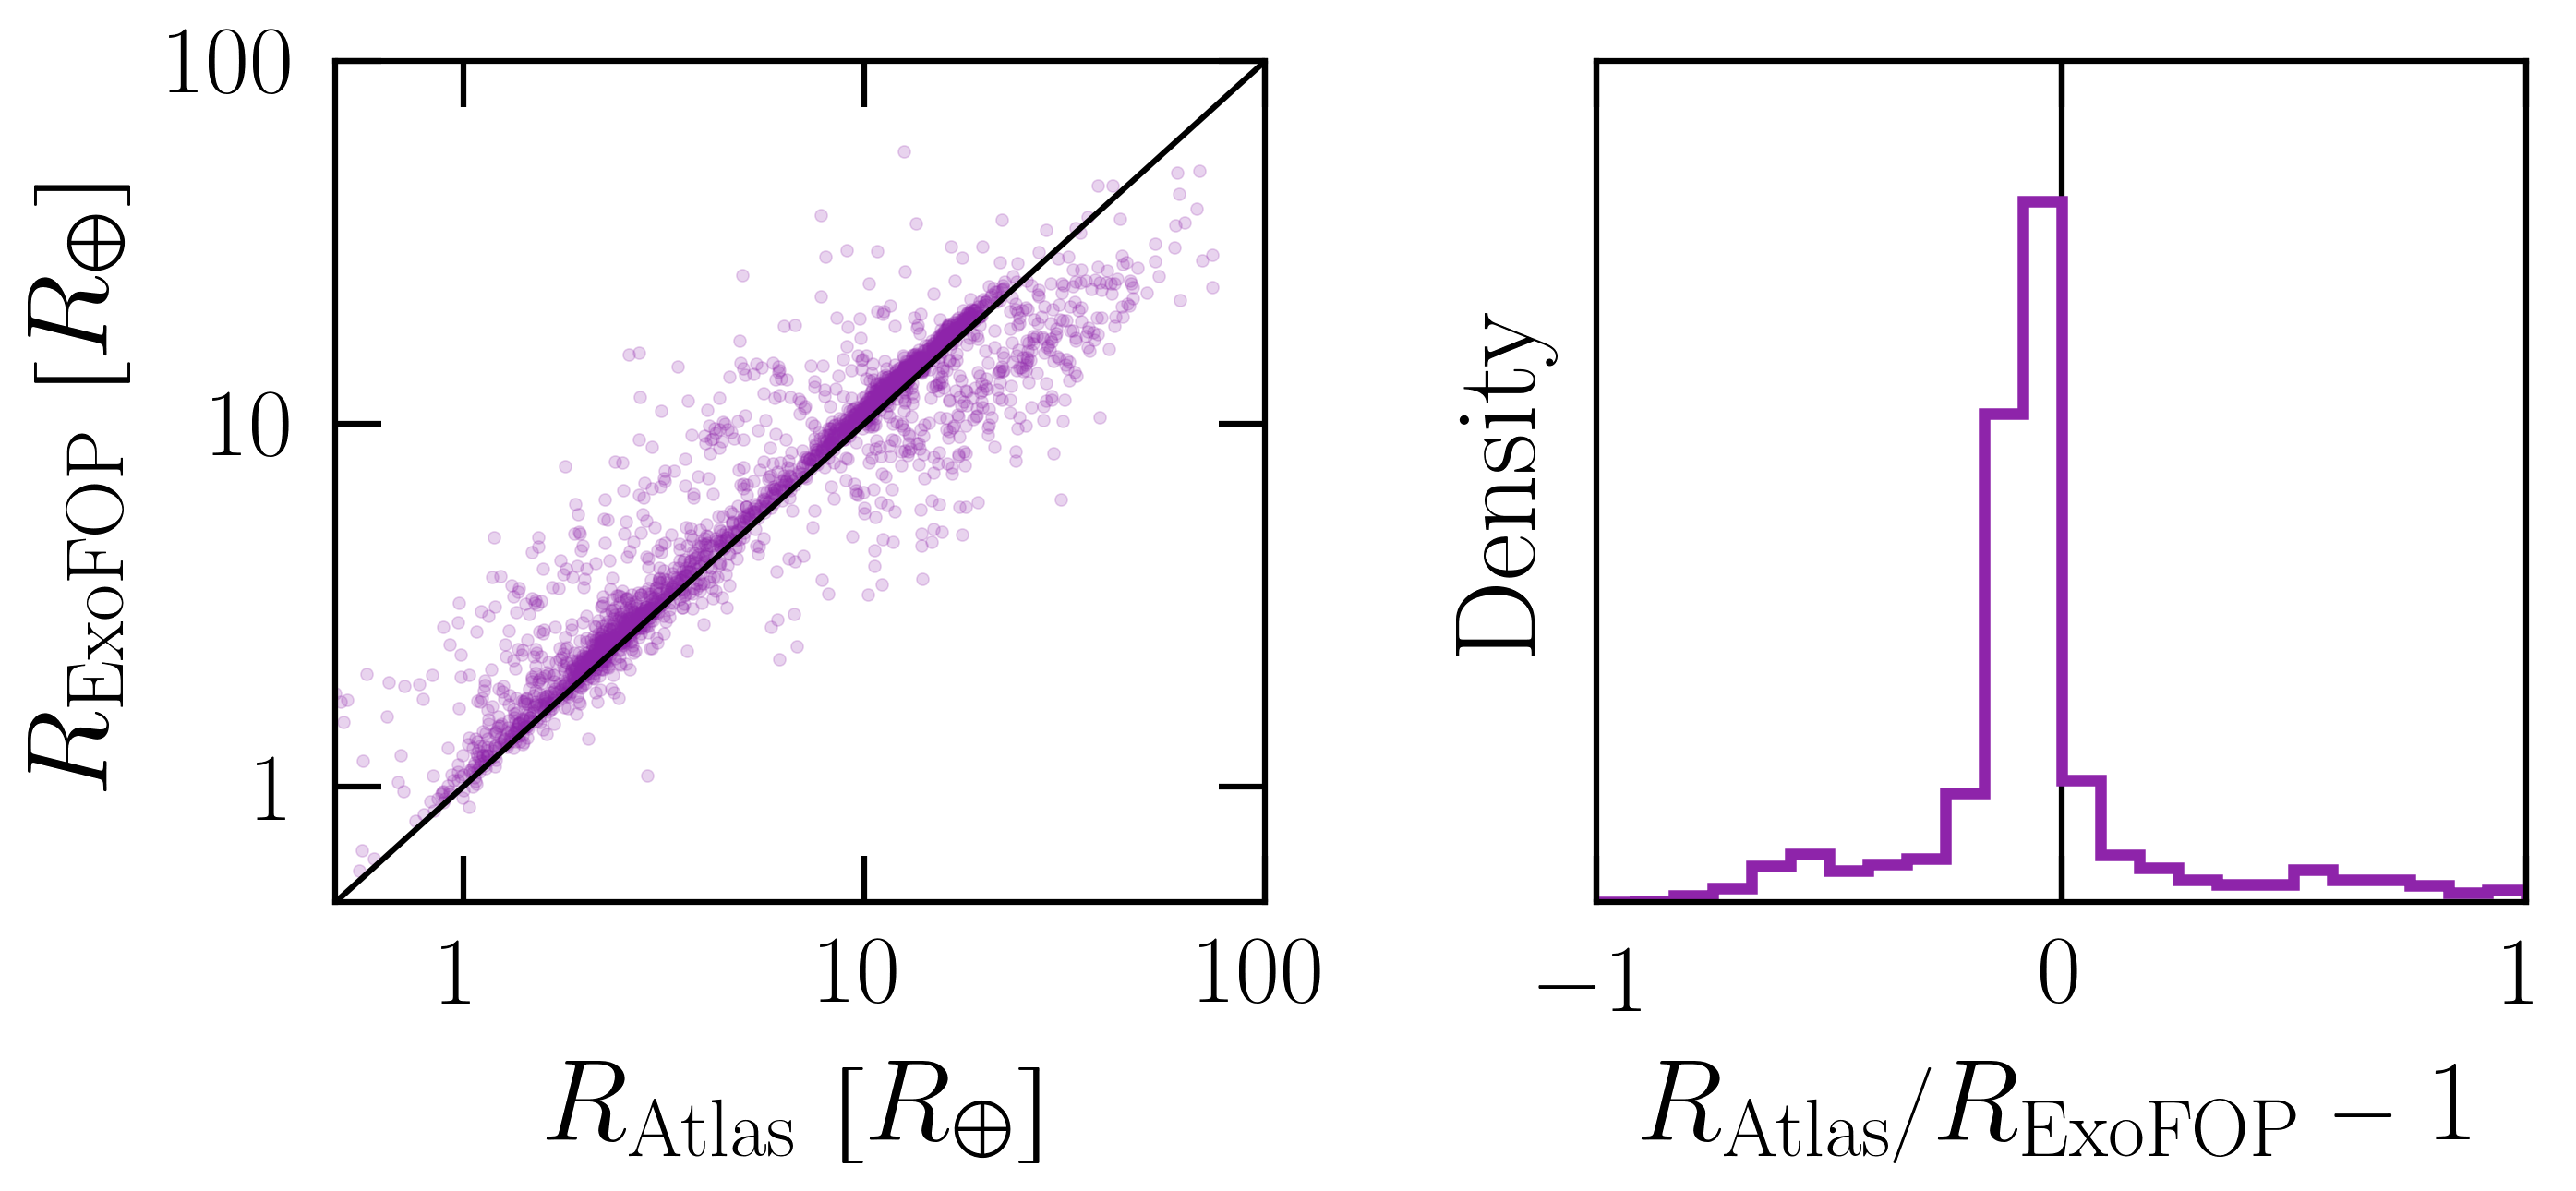
\includegraphics[width=\linewidth]{figures/radius_error.png}
  \caption{\textbf{Main caption:} . The black line shows the one- to-one correspondence. As expected, there is good agreement between the two methods although the MCMC values are systematically smaller than those found by DV. The largest disagreement is typically for KOIs with large fit values for impact parameter. }
  \label{fig:}
\end{figure}





\section{Discussion}\label{sec:conclusion}
We present for the first time a catalog of Bayesian posterior samples for the 2-minute cadence TOIs from 2018-2022.
Some words about results.
Some stuff about difficulty sampling grazing systems.
Errors when SPOC estimates are off.
We expect the remainder of the \tess\ extended mission will complete by September 2023, at which point an updated catalog will be produced.

Vetters can identify false positive TCEs by a few tell- tale signs: a visible secondary eclipse which cannot phys- ically be planetary in nature; a mismatch between odd and even transit depths caused by a stellar binary at twice the indicated period; a shift of the centroid to another nearby star; and increasing transit depth with aperture size, indicative that a signal is from an object nearby on the sky and not the suspected target star.

Lots of manual vetting requiured to promote TCE to TOI. In the future this work can help with that process.


\section{Data and software availability}\label{sec:data}
Software to carry out this analysis on github.

Data for analysis obtained from exofop, MAST. 

Our analysis data products are availible on the website.

Can be downloaded from the website.

Alternatively, if a user installs the `tess-atlas` python package, they can use the command line interface to download the data and notebooks.

download toi to get one analysis
download population summary
download all fits


%%%%%%%%%%%%%%%%%%%%



\section*{Acknowledgments}{

We would like to thank xyz.
Ozgrav, Flatiron, NECTAR, ADACS, David Liptai
Work was started during `online.tess.science`

This work has used the TIC through the TESS Science Office’s target selection working group (architects K. Stassun, J. Pepper, N. De Lee, M. Paegert, R. Oelkers).

This research has made use of the NASA Exoplanet Archive, which is operated by the California Institute of Technology, under contract with the National Aeronautics and Space Administration under the Exoplanet Exploration Program.

This work made use of the \tess\ catalog on ExoFOP

Total compute time for this work \red{\cpuHrs} \alltodo{get more accurate compute time (this is an overestimate)}. CO$_2$ emission amount for this work would be XX, however as OzStar uses wind energy this has a negligible carbon footprint.

}

\vspace{5mm}
\facilities{\tess, \gaia, \kepler, Exoplanet Archive, etc.}

\software{
astropy \citep{Astropy-Collaboration:2013,Astropy-Collaboration:2018},
exoplanet,
lightkurve,
starry,
celerite2,
pymc3,
numpy,
scipy,
pandas,
matplotlib,
corner,
sphinx,
}


% ADS bibliography link
% https://ui.adsabs.harvard.edu/user/libraries/_DyLS4HbTY-eJIMBiFUdxw
\bibliography{atlas}{}
\bibliographystyle{aasjournal}

%%%%%%%%%%%%%%%%%%%%%%%%%%%%%%%%%%%%%%%%%%%%
\appendix

\section{Transit model parameterisation details}\label{apdx:model_details}

\paragraph{Transit depth}
The small planet approximation of the transit depth, $\delta=k^2$, is useful as it is directly invertible (conditioned on the limb darkening parameters and impact parameter).
However, the parameterisation restricts the model to non-grazing transits with impact parameter $|b| \le 1$.
Accepting this restriction, we can compute the approximate transit depth for a limb darkened light curve by assuming that the intensity of the star is uniform under the disk of the planet.
For quadratic limb darkening, the intensity profile is
\begin{equation}
  I(r) = 1 - u_1\,[1 - \mu(r)] - u_2\,[1 - \mu(r)]^2
\end{equation}
where $\mu(r) = \sqrt{1 - r^2}$.
The ratio of the occulted flux to the total stellar flux when the transit is deepest ($r = b$) is \citep[the same results are discussed by][]{Mandel:2002,Csizmadia:2013, Agol:2020:AJ}
\begin{eqnarray}
  \delta &\approx& \frac{\int_0^k\,2\,\pi\,r\,I(b)\dd r}{\int_0^1\,2\,\pi\,r\,I(r)\dd r} \nonumber\\
  &=& \frac{k^2\,\left(1 - u_1\,[1 - \mu(b)] - u_2\,[1 - \mu(b)]^2\right)}{1 - u_1/3 - u_2/6}\quad.
\end{eqnarray}
Therefore, since $k$ must be positive, we have a one-to-one transformation between $\delta$ and $k$ conditioned on impact parameter $|b| \le 1$ and the limb darkening coefficients.
It is also important to include the Jacobian factor so that fitting in $\delta$ doesn't introduce a strange prior on $r$.
In this case, the relevant factor is
\begin{equation}
  \left|\frac{\dd k}{\dd \delta}\right| = \left|\frac{1 - u_1/3 - u_2/6}{2\,k\,\left(1 - u_1\,[1 - \mu(b)] - u_2\,[1 - \mu(b)]^2\right)}\right| \quad.
\end{equation}


\paragraph{Transit times}
To expedite the analysis, we assume that the \exofop\ period and phase of the orbit are sufficiently accurate to fit only the data nearby the anticipated transit times (with some buffer, $\pm2\tau$) and disregard the remaining data.
This implies that the number of periods $N_P$ in the TESS observational baseline is exact and the transits must occur within the data cutouts.
This can be difficult to enforce---especially for low signal-to-noise transits.
A good approximation can be achieved by fitting for two reference transit times, $t_{\rm min}$ and $t_{\rm max}$, with a fixed number of periods, $N_P$, between them, instead of a single reference time and the period.
Then the implied period can be computed as $P = (t_{\rm max} - t_{\rm min}) / N_P$.
Importantly this does not change the prior on $P$ and $t_0$ since the Jacobian is a constant $1/N_P$.


\paragraph{Transit duration}
The transit duration $\tau$ is better constrained than the orbit's semi-major axis, $a$ the so it can be better as a fit parameter.
For a circular orbit, the transit duration is \citep{Winn:2010}
\begin{equation}
  \tau = \frac{P}{\pi}\,\sin^{-1}\left( \frac{\sqrt{(1 + k^2) - b^2}}{a\,\sin i} \right) \quad.
\end{equation}
Rearranging this, we find
\begin{equation}
  a^2\,\sin^2 i\,\sin^2\left(\frac{\pi\,\tau}{P}\right) = (1 + k^2) - b^2 \quad.
\end{equation}
Then, using the fact that $\cos^2 i = b^2 / a^2$, we find
\begin{equation}
  a^2 = \frac{(1 + k)^2 - b^2\,\cos^2\phi}{\sin^2\phi}
\end{equation}
for $\phi = \pi\,\tau / P$.
And the Jacobian is
\begin{eqnarray}
  \frac{\dd a}{\dd \tau} &=& \frac{\pi\,\cos \phi}{a\,P\,\sin^3 \phi}\,\left[b^2 - (1 + k)^2\right] \quad.
\end{eqnarray}

Finally, from the period and semi-major axis, we can compute the implied stellar density (under this assumption of a circular orbit)
\begin{equation}
  \rho_\mathrm{circ} = \frac{3\,\pi\,a^3}{G\,P^2} \quad.
\end{equation}
It is important to note that this is not necessarily the same as the actual stellar density and that, in a multi-planet system, this implied density won't be the same for each planet \citep[see, for example,][]{Dawson:2012, Kipping:2012}.



\end{document}
